\section{Echo Experiments}
\label{results}

%Our experiments were designed to test whether or not Echo exhibits
%a scaling relation similar to that observed in natural ecologies.
%Further, by asking whether
%$z\approx 1/4$, we can formally compare the quantitative behavior of our
%model with that of empirical communities.  

Our experiments were designed to test how closely Echo exhibits
canonical Preston distributions and species-area scaling relations.
We consider these experiments to be one step in testing whether Echo
exhibits ecologically plausible dynamics.  
To test whether observed diversity patterns in Echo result from random
processes or from selective pressures, we compare the
behavior of the original Echo model with that of a neutral model
that replaces the Echo interaction rules with random interactions
between agents.  Thus, comparing the original and neutral versions of
Echo allows us to ask whether tag-mediated interactions are necessary
to produce observed patterns of diversity.
 
\subsection{Simulation Parameters}

% this figure was generated with xfig 3.1 .  the source file is at:
% algodones.unm.edu:~phraber/projects/modeling-paper/antcatfly.fig
\begin{figure}[t!]
\begin{center}
\leavevmode
\ifepsf
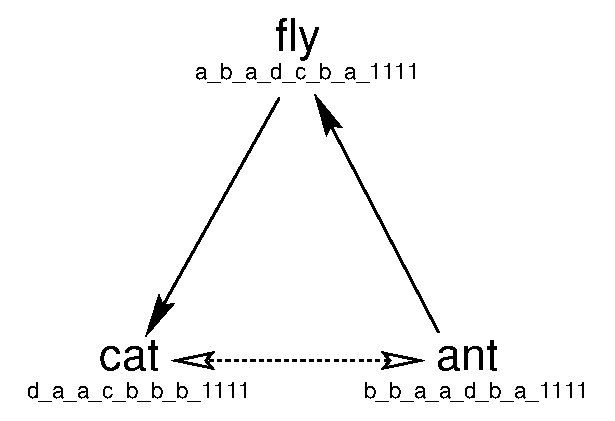
\epsfig{file=figures/antcatfly.eps}
\else
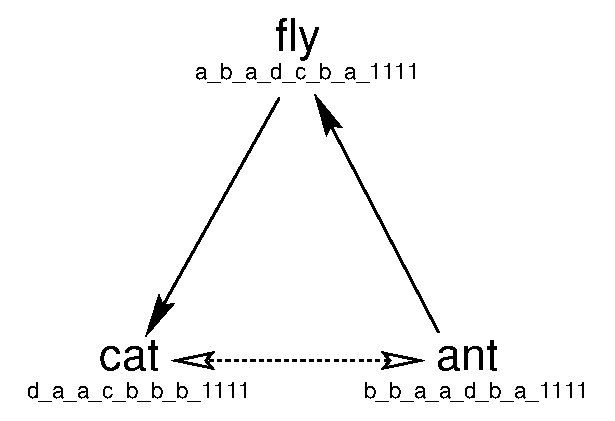
\psfig{file=figures/antcatfly.eps}
\fi
\caption{Echo agents initially present in experiments described in
this section.  Interactions among ants, caterpillars (``cat'') and
parasitic flies are coded by agent genotypes.  Open arrows indicate
mutualistic trade between ants and caterpillars.  Closed arrows
indicate direction of an attack in combat (flies attack caterpillars;
ants attack flies).  The genotype of each agent is indicated with 
loci in the following order: offense tag, defense tag, mating tag,
combat condition, trading condition, mating condition, trading resource,
and uptake mask.
\label{fig:antcatfly}}
\end{center}
\end{figure}

We have run experiments with a variety of initial conditions.  The two
most common setups are as follows: (1) start with a single founding
agent that is one mutation away from trading, fighting, and mating with 
itself, and (2) start with a small set of hand-designed agent types
that encode some interaction pattern of interest.  The experiments
reported here all use the second setup, consisting of three agent
types that form a trophic triangle.  However, we get similar results
when the first style of initial condition is used (data not shown).

Figure~\ref{fig:antcatfly} illustrates the initial conditions
used in the experiment detailed in this section.  This ant,
caterpillar, fly interaction network was described by Holland
\cite{Holland9?} [and is based on observations by Holldobler and
Wilson \cite{HolldoblerAndWilson90}].  The caterpillars secrete a
nectar which is collected by the ants.  In exchange, ants nurture
the caterpillars.  Parasitic flies attempt to consume caterpillar
larvae, while the ants defend their symbionts.  Initially, each site
in a world has ten agents of each genotype present, with ten letters
of each resource type in reserve.  No mating occurs initially, though
mutation could produce such an interaction during simulation.

% this paragraph used to be first in this subsection but PTH moved
% it here
The parameters used in our experiment are shown in
Table~\ref{tab:simulation-parameters}.  We vary the area
by defining worlds with multiple identical sites.  Agents
which fail to acquire resources during a time step are allowed to
migrate to one of the site's four neighbors to the north, south, east
or west.  Periodic boundary conditions are imposed on worlds
comprised of 1, 4, 16 or 64 sites.  Thus, agents live in toroidal
worlds of a fixed size; this is roughly analagous to living on an 
island of given area.  Independent simulations were run for both 1,000
and 10,000 iterations.

\begin{table}[t!]
\begin{center}
\begin{tabular}{|l|c|} \hline
Parameter & Value \\ \hline
Number of Resources & 4 \\
Trading Fraction & 0.5 \\
Interaction Fraction & 0.02 \\
Self Replication Fraction & 0.5\\
Self Replication Threshold & 2\\
Taxation Probability & 0.1 \\ \hline
Mutation Rate & 0.02 \\
Crossover Probability & 0.07 \\
Random Death & 0.0001 \\
Initial Vector & 10 \\
Production Vector & 10 \\
Maximum Vector & 100 \\
Maintenance Vector & 1 \\ \hline
\end{tabular}
\end{center}
\caption{Parameters used for Echo experiments described in text.  See
Section~\protect\ref{echo-structure} for a detailed description of each
parameter.  World-level parameters are above the line; site-specific 
parameters are below.  Resource parameters are indicated as vectors.  
In our experiments these values are equal for all four resources.
\label{tab:simulation-parameters}}
\end{table}

\subsection{The Neutral Model}
\label{neutral-model}

Neutral models are used in biology to evaluate what mechanisms are
necessary to produce a phenomenon of interest
\cite{Caswell76,NiteckiAndHoffman87}.  Here we are interested whether
tags and conditions affect patterns of diversity in Echo populations.
Non-random mating, competition or predation, and direct or indirect
mutualisms are all believed to regulate species diversity in
ecological communities.  The question for both Echo and the real world
is whether such mechanisms are 
necessary to produce patterns such as the species-area scaling
relation.  The neutral model we implemented substitutes the tag-based
interactions described in Section~\ref{agent-agent} with random
interactions.  When two agents are chosen to interact, the decision of
whether they will fight, trade, or mate is based on random tosses of a
biased coin, rather than string-matching criteria.  This adjustment 
is analagous to an ecology in which species interact with one another
randomly.  Aside from this modification, all other bookkeeping (i.e.,
resource assimilation, self-replication, migration, taxation, and
random death) is performed identically in both models.

%[MERGE IN WITH THE PREVIOUS PARAGRAPH]
%The neutral version of Echo replaces tag-based interactions with
%random interactions (see section~\ref{neutral-model}).  Thus, the
%neutral model removes the effect of the genome on agent-agent
%interactions.  If both versions of Echo exhibit the same patterns seen
%in nature, then one of two conclusions can be drawn.  Either Echo is
%not a minimal model (that is, not all of its mechanisms are needed to
%produce the relevant behaviors), or explanations in the ecological
%literature have posited more complexity than necessary
%\cite{Caswell76,ConnorSimberloff79,NiteckiAndHoffman87} to account
%for observed patterns.  [PETER: I still don't understand this second
%point] 
% PTH says: If the Preston distribution results from random processes,
%           why infer that other process (e.g., competition,
%           mutualisms, etc.) are responsible for the pattern?
%           By parsimony, random processes alone are necessary to produce
%           the pattern.

\begin{table}[t!]
\begin{center}
\begin{tabular}{|c||c|c|c||c|} \hline
& {\sc Combat} & {\sc Trade} & {\sc Mating} & {\sc Total} \\
& $P_{combat}\cdot P_{escape}$ & $(1-P_{combat})\cdot P_{trade}$ & $(1-P_{combat})\cdot P_{mating}$ & $P_{int}$ \\ \hline 
Neutral model & $1/4 \cdot 1/2$ & $(1-1/4) \cdot 1/8$ & $(1-1/4) \cdot 1/8$ & $10/32$ \\ \hline
Original model & $1/m^n \cdot P_{escape}$ & $(1-P_{combat})(1/m^n)^2$ & $(1-P_{combat})(1/m^n)^2$ & $P_{int}$ \\ \hline
n=0 & $1/1 \cdot 1/2$ & $(1-1) (1/1)^2$ & $(1-1) (1/1)^2$ & $1/2$ \\
n=1 & $1/4 \cdot 1/2$ & $(1-1/4) (1/4)^2$ & $(1-1/4) (1/4)^2$ & $7/32$ \\
n=2 & $1/16 \cdot 1/2$ & $(1-1/16) (1/16)^2$ & $(1-1/16) (1/16)^2$ & $\approx 1/32$ \\ \hline

%Neutral model & $\frac{1}{4} \times \frac{1}{2}$ & $(1-\frac{1}{4}) \times \frac{1}{8}$ & $(1-\frac{1}{4}) \times \frac{1}{8}$ & $\frac{10}{32}$ \\ \hline
%Original model & $\frac{1}{m^n} \times P_{escape}$ & $(1-P_{combat})(\frac{1}{m^n})^2$ & $(1-P_{combat})(\frac{1}{m^n})^2$ & $P_{int}$ \\ \hline
%n=0 & $\frac{1}{1} \times \frac{1}{2}$ & $(1-1) \times (\frac{1}{1})^2$ & $(1-1) \times (\frac{1}{1})^2$ & $\frac{1}{2}$ \\
%n=1 & $\frac{1}{4} \times \frac{1}{2}$ & $(1-\frac{1}{4}) \times (\frac{1}{4})^2$ & $(1-\frac{1}{4}) \times (\frac{1}{4})^2$ & $\frac{7}{32}$ \\
%n=2 & $\frac{1}{16} \times \frac{1}{2}$ & $(1-\frac{1}{16}) \times (\frac{1}{16})^2$ & $(1-\frac{1}{16}) \times (\frac{1}{16})^2$ & $\approx \frac{1}{32}$ \\ \hline
\end{tabular}
\end{center}
\caption{Comparison of probability values for interactions between
agents in neutral and original models.  The alphabet
size ($m$) for genotypes is the number of resources used (4 for our
simulations).  For the original model, probabilities are shown for
conditions of length ($n$) 0, 1 and 2.
\label{tab:neut-model-params}}
\end{table}

Parameters for the neutral model were chosen to produce the same
interaction probability between two randomly selected agents 
as in the original Echo model.  The chance an interaction will
occur between two randomly chosen agents is the sum of the
probabilities that combat, trade, or mating will occur
(Table~\ref{tab:neut-model-params}).  For the neutral 
model, probabilities of combat, trade, and mating were set at $1/4$,
$1/8$, and $1/8$, respectively.

As we described earlier, if an agent is attacked by another agent in
combat, the attacked agent is given a chance to flee from the
attacker.  The probability of escape equals the probability of losing
in combat.  In the neutral model, an agent will escape attack with a
probability of $1/2$.  In the neutral model, the chance of
being attacked and defeated is the product of the probability of
combat and the chance of escape ($1/4 \cdot 1/2 = 1/8$).  Thus, the
 probability that any interaction will occur between two selected 
agents in the neutral model is $10/32$.

%In the original model, the probability of escape varies with scores from 
%matching alleles in offense and defense tags in the combat matrix.
%The combat matrix used in our experiments assigns equal scores to
%matches at all loci, so the probability of escape from combat for any
%two agents with loci of the same length will be $1/2$.
In the original model, the probability any interaction will occur is
based on the chance of randomly matching a condition as a prefix of a
tag.  For mating and trade to happen, combat must not occur,
and each agent must match its condition as a prefix of the other's tag.
Denoting $n$ as the mean length of the conditions in agents' genomes,
we calculate the probability of any interaction occurring between two
agents in Echo to be $P_{int} = 1/2$ for $n=0$, $7/32$
for $n=1$, and $\approx 1/32$ for $n=2$.  For our experiment,
the mean length of conditions in the original model was 0.98, and
lengths of conditions for individual genotypes ranged from 0 to 6
(data not shown).  We conclude that the average interaction
probability is equal in the neutral and original versions of Echo.

\subsection{Experimental Design and Data Analysis}
\label{data-analysis}

Our experiments were designed to test whether or not $S_{tot} = cA^z$
in both the original and neutral versions of Echo.  To test this,
%whether $S \sim A^{1/4}$, 
we used a $4 \times 2 \times 2$ factorial
design, with $20$ replicates for each combination of world area (1, 4,
16, or 64 sites), number of iterations ($10^3$ or $10^4$ iterations),
and model type (original or neutral model).  For each replicate
population, we recorded $S_{tot}$ (number of species), $N_{tot}$
(number of individuals), and $N_{max}/N_{tot}$ (an index of dominance,
the fraction of the population represented by the most abundant species
\cite{Pielou77}).  We also calculated the mean number of species and
individuals per site ($S/$site and $N/$site).
Although other definitions of species in Echo have been considered
(see \cite{ForrestAndJones94}), in this study, a species is defined as
a unique genotype.  
%To test for significant treatment effects, we used two-way analysis
%of variance (ANOVA) \cite{Lindman74,Potvin93} 
%on three response variables: mean $S$ and $N$ per site, and dominance.
%Separate analyses were conducted for runs lasting $10^3$ and $10^4$
%iterations.  
% For a
% given set of treatment factors (the statistical ``model''), ANOVA
% breaks down variance into within treatment and between treatment
% components, then calculates a test statistic ($F$) from the ratio of
% between group error (``model'' sum of squares) to within group error
% (error sum of squares).  If this test value corresponds to a
% probability of 95\% or greater significance, we conclude the model
% accounts for more variation than by chance.  We tested models for all
% treatment factors (model type, area, and time) and their interactions.
% ANOVA was perfomed in SAS \cite{SAS85}.
% {\it Post hoc} comparisons were made for the area factor, to distinguish
% which areas exhibited different responses.  The {\it post hoc}
% comparisons were made with a Bonferroni correction to the significance
% test.  The Bonferroni correction controls experimentwise type I error
% rate, and is a conservative test for differences among treatment
% levels \cite{Philippi93}.

We used multiple regression to compare coefficients of species-area
functions in the original and neutral models.  
%Regression calculations were performed in SAS on the
%log$_2$-transformed species counts, and used backwards elimination to
%build the best regression equation.  Backwards elimination is an
%iterative procedure which fits a regression to all variables, then
%successively eliminates variables which do not contribute to the
%regression equation.  
The full regression equation was in the form
$\widehat{S_{tot}} = (\beta _1 + \beta _2)A^{(\beta _3 + \beta _4)} +
\epsilon$ for the original model and $\widehat{S_{tot}} = \beta _1
A^{\beta _{3}} + \epsilon$ for the neutral model.  A variable was
eliminated from our regression equation if it had less than 90\%
probability of being significantly different from 0.  To
interpret these regression equations, note that eliminating $\beta _4$
from the best regression equation implies that model type has no
significant effect on $z$, but that $\beta _3$ can be used to predict
$z$ for both models.  Similarly, eliminating $\beta _2$ implies that
model type has no significant effect on $c$, and can be predicted by
$\beta _1$ alone.  The $\epsilon$ term describes residual error.
Separate equations were built for runs of $10^3$ and $10^4$ iterations.

\subsection{Results}

% Preston curves
% this figure came from
% algodones:/landscape/users/phraber/projects/modeling-paper/preston-plots.  
% data were generated with the script sfi:~pth/projects/Echo/bin/preston
% for the following runs:
% model   time    area    seed            outfile
% orig    3       1       519477386       preston-a
% orig    4       64      237813364       preston-b
% neut    3       1       179905860       preston-c
% neut    4       64      87600382        preston-d
\begin{figure}[t!]
\begin{center}
\leavevmode
\ifepsf
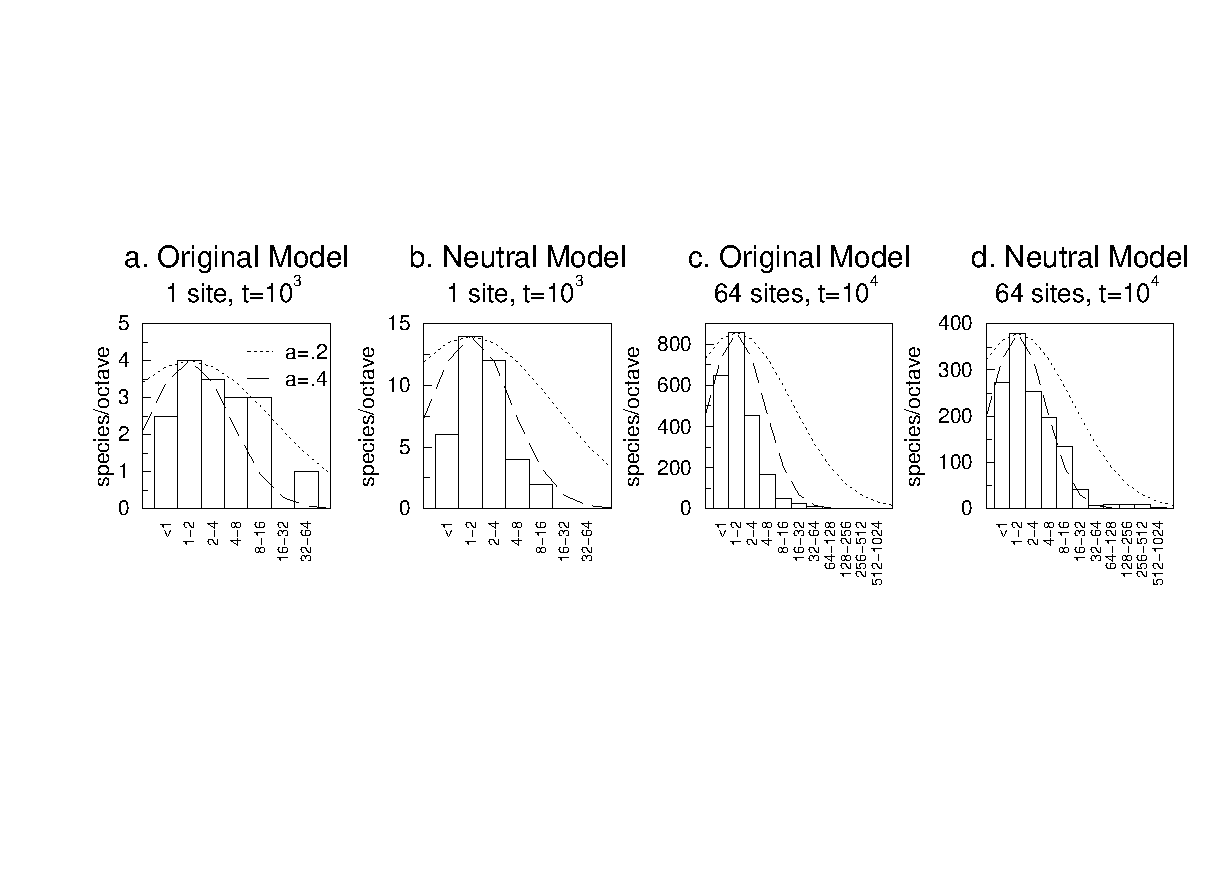
\epsfig{file=figures/preston-curves-h.ps,height=1.5in,width=6in,bbllx=0,bblly=140,bburx=620,bbury=350}
\else
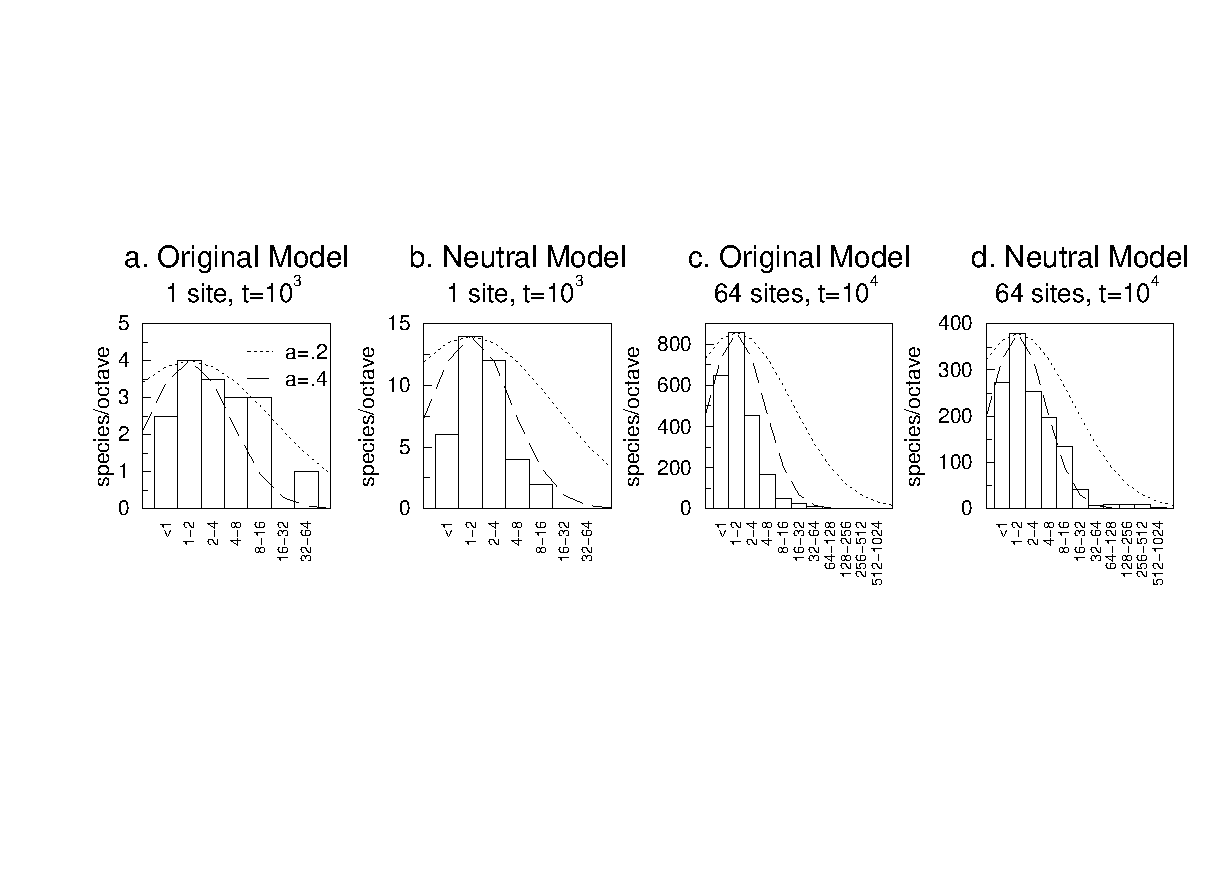
\psfig{file=figures/preston-curves-h.ps,height=2in,width=6in}
\fi
\caption{Preston curves from four Echo populations.  See
  section~\protect\ref{preston-distribution} for a description of
  Preston curves.  Populations are from original (a, c) and neutral
  (b, d) models, either for a one-site world at 1000 iterations
  (a, b), or for a 64-site world at 10,000 iterations (c, d).  Each
  population was randomly chosen from 20 replicates.  Expected values
  under Preston's canonical hypothesis are plotted as dotted and
  broken lines, for $a=.2$ and $a=.4$, respectively.
\label{fig:preston-curves}}
\end{center}
\end{figure}

Preston curves from typical populations are shown in
Figure~\ref{fig:preston-curves}, and additional data are reported in
\cite{ForrestAndJones94}.  Populations from both the original and
neutral model are plotted, for short runs in small worlds, and for
longer runs in larger worlds.  Distributions expected under Preston's
canonical hypothesis are plotted for comparison.  These data suggest
the pattern of genome abundances in Echo populations qualitatively
resembles Preston's log-normal distribution, although there are some
differences.  We have observed this general pattern in a wide variety
of Echo runs under a wide variety of different parameter settings and
initial conditions.  As we discussed earlier, we do not believe that a
careful quantitative comparison is possible, so the remainder
of our experiment focusses on the species-area scaling relation.

% ANOVA response variables (bar plots)
% this figure came from algodones:/landscape/users/phraber/projects/modeling-paper/sas/anova/means/histo.ps
\begin{figure}[t!]
\begin{center}
\leavevmode
\ifepsf
\epsfig{file=figures/anova-response-vars-h.ps,height=2.5in,width=6in,bbllx=80,bblly=330,bburx=730,bbury=780}
\else
%\psfig{file=figures/anova-response-vars-h.ps,height=2.5in,width=6in,bbllx=80,bblly=330,bburx=730,bbury=780}
\psfig{file=figures/anova-response-vars-h.ps,height=2.5in,width=6in}
\fi
\caption{Response variables from simulations of $10^3$ iterations
  (a, b, c) and $10^4$ iterations (d, e, f).  Species richness per site
  (a, d), population size per site (b, e) and dominance (c, f) are
  plotted as a function of area.  Solid (black) bars are from the
  original model and unfilled (white) bars are from the neutral model.
  Each bar represents a mean from twenty replicates.  Error bars
  indicate one standard deviation.
\label{fig:anova-response-vars}}
\end{center}
\end{figure}

In simulations lasting $10^3$ iterations, the neutral model
has more species per site than the original model.
(Figure~\ref{fig:anova-response-vars}a, b, c).  Increasing area
decreases number of species per site in the neutral model and
decreases dominance in the original model.  Number of individuals per
site is not affected by model type or area of the world.  

Variances in all response variables are greater in longer runs than
in shorter runs (Figure~\ref{fig:anova-response-vars}d, e, f).
Dominance and number of species per site do not differ with model type,
but the neutral model has more individuals per site than the
original model.  Increasing area increases the number of individuals per
site, and decreases dominance and number of species per site.

%[PETER: please explain someplace what you mean by dominance.-done]
%In the test for a species-area scaling relation, the analysis of
%variance on simulations lasting $10^3$ iterations indicates that the
%original and neutral versions of Echo have significantly different
%means for number of species per site and number of individuals per
%site (Table~\ref{tab:anova-results-t3},
%Figure~\ref{fig:anova-response-vars}a, b).  Dominance does not differ
%with model type (Table~\ref{tab:anova-results-t3},
%Figure~\ref{fig:anova-response-vars}c).  Increasing area has
%significant effects on mean species per site and dominance, but not on
%the number of individuals per site.  Treatment interaction effects
%[PETER: what does ``treament interaction effects'' mean?] are detected
%for species per site and dominance (Table~\ref{tab:anova-results-t3}).
%For runs lasting $10^4$ iterations, variances in response variables
%are greater (Figure~\ref{fig:anova-response-vars}d, e, f).  Model type
%has a significant effect on $N$/site only
%(Table~\ref{tab:anova-results-t4},
%Figure~\ref{fig:anova-response-vars}e).  
%Varying area has significant effects on all three response variables
%(Table~\ref{tab:anova-results-t4},
%Figure~\ref{fig:anova-response-vars}d, e, f).  
%Effects of a model type by area interaction have a marginally
%significant effect on $S$/site (Table~\ref{tab:anova-results-t4}).
%[PETER: need a little more prose here explaining all this.]
%[STEPH: let's combine these two tables, make them more compact, and
%do them in the same style as the other tables]
% ANOVA tables
% these data come from algodones:/algodones/users/phraber/projects/modeling-paper/sas/anova/anova-t3-not-log-xformed.lst
%\begin{table}[btp!]
%\caption{ANOVA results from simulations lasting $10^3$ iterations.
%Treatments are model type
%(original or neutral model) and world area (1, 4, 16 or 64 sites).
%Response variables are mean number of species per site, mean number of
%individuals per site, and dominance.  Asterisks indicate significance
%of the $F$ test ($P$).  [PETER: explain all headings---I couldn't understand
%this table.]
%% Tables:
%% ANOVA tables
%\label{tab:anova-results-t3}}
%\begin{center}
%\begin{tabular}{lrrrl} \hline \hline
%{\sc Source} & df & ss (I) & $F$ & \\ \hline
%\multicolumn{5}{c}{{\sc Mean S per site}} \\
%{\sc Type}                &   1 &  3107.6 &  294.66 & **** \\
%{\sc Area}                &   3 &  2489.4 &   78.68 & **** \\
%{\sc Type$\times$Area}    &   3 &   672.2 &   21.25 & **** \\
%{\sc Error}               & 152 &  1603.1 & & \\ \hline
%\multicolumn{5}{c}{{\sc Mean N per site}} \\
%{\sc Type}                &   1 &  125.8  &  15.59 & **** \\
%{\sc Area}                &   3 &   11.7  &   .48 & \\
%{\sc Type$\times$Area}    &   3 &   37.0  &   1.53 & \\
%{\sc Error}               & 152 & 1226.9  & & \\ \hline
%\multicolumn{5}{c}{{\sc Dominance}} \\
%{\sc Type}                &   1 & .0092 &    5.21 & \\
%{\sc Area}                &   3 & .3099 &   58.67 & **** \\
%{\sc Type$\times$Area}    &   3 & .1969 &   37.29 & **** \\
%{\sc Error}               & 152 & .2676 & & \\ \hline
%** $P \le .01$, *** $P \le .001$, **** $P \le .0001$.
%\end{tabular}
%\end{center}
%\end{table}
%% these data come from algodones:/algodones/users/phraber/projects/modeling-paper/sas/anova/anova-t4-not-log-xformed.lst
%\begin{table}[btp!]
%\caption{ANOVA results from simulations lasting $10^4$ iterations.
%  Treatments and response variables are as in
%  Table~\protect\ref{tab:anova-results-t3}
%\label{tab:anova-results-t4}}
%\begin{center}
%\begin{tabular}{lrrrl} \hline \hline
%{\sc Source} & df & ss (I) & $F$ & \\ \hline
%\multicolumn{5}{c}{{\sc Mean S per site}} \\
%{\sc Type} & 1 & 10.1 & 0.05 & \\
%{\sc Area} & 3 & 9305.8 & 15.28 & **** \\
%{\sc Type$\times$Area} & 3 & 3192.7 & 5.24 & ** \\
%{\sc Error} & 152 & 30863.1 & & \\ \hline 
%\multicolumn{5}{c}{{\sc Mean N per site}} \\
%{\sc Type} & 1 & 52531.9 & 31.24 & **** \\
%{\sc Area} & 3 & 87099.5 & 17.27 & **** \\
%{\sc Type$\times$Area} & 3 & 15089.7 & 2.99 & \\
%{\sc Error} & 152 & 255562.6 & & \\ \hline
%\multicolumn{5}{c}{{\sc Dominance}} \\
%{\sc Type} & 1 & 0.0177 & 2.16 & \\
%{\sc Area} & 3 & 0.4259 & 17.31 & **** \\
%{\sc Type$\times$Area} & 3 & 0.0164 & 0.66 & \\
%{\sc Error} & 152 & 1.2468 & & \\ \hline
%** $P \le .01$, *** $P \le .001$, **** $P \le .0001$.
%\end{tabular}
%\end{center}
%\end{table}
% END ANOVA tables

%regression coefficients
% these data come from algodones:/algodones/users/phraber/projects/modeling-paper/sas/SA/SvA-full.lst
\begin{table}[btp!]
\caption{Coefficients from multiple regression analysis.  Treatments
  of different durations ($T$) were analyzed separately.  Parameter
  estimates are shown for the best regression equation, after backwards
  elimination of parameters with $P>0.10$.  See
  section~\protect\ref{data-analysis} for a description of the multiple
  regression equations.  All parameters are
  significant at $P\le .001$.
\label{tab:regress-coeffs}}
\begin{center}
\begin{tabular}{|c|c||cc|cc||c|} \hline
\emph{T} & \emph{n} & $\beta _1$ & $\beta _2$ & $\beta _3$ & $\beta _4$ & $r^2$ \\
 & & \multicolumn{2}{c|}{($c$)} & \multicolumn{2}{c||}{($z$)} & \\ \hline \hline
$10^3$ & 160 & 5.39 & -.62 & .87 & .08 & .995 \\
$10^4$ & 160 & 5.78 & -.62 & .70 & .23 & .877 \\ \hline
\end{tabular}
\end{center}
\end{table}

A scaling relation
describes the species-area function in both models at $10^3$
iterations, and in the original model at $10^4$ iterations
(Figure~\ref{fig:species-area-curves}).  Mild curvilinearity might
be present in the species-area function for the neutral model at
$10^4$ iterations.  With this minor exception, we note that both
models demonstrate the hypothesized scaling relation.  Multiple
regression analyses indicate all terms in the full regressions
equation are statistically significant
(Table~\ref{tab:regress-coeffs}).  That is, we reject with more than
99\% confidence the null hypotheses that $\beta _2 = 0$ and $\beta _4
= 0$.  Thus, values of $c$ and $z$ for the original and neutral models
differ significantly.  Actual values for $z$ at $10^3$ iterations are
$0.95$ and $0.87$ for the original and neutral models, respectively 
(Figure~\ref{fig:species-area-curves}a).
Simulations of $10^4$ iterations yield $z$ values of $0.93$ and $0.70$ 
for original and neutral models (Figure~\ref{fig:species-area-curves}b).  

%SA curves
% this figure came from algodones:/landscape/users/phraber/projects/modeling-paper/sas/SA/SA.ps
\begin{figure}[t!]
\begin{center}
\leavevmode
\ifepsf
\epsfig{file=figures/species-area-curves-h.ps,height=3in,width=6in,bbllx=80,bblly=350,bburx=740,bbury=840}
\else
%\psfig{file=figures/species-area-curves-h.ps,height=3in,width=6in,bbllx=80,bblly=350,bburx=740,bbury=840}
\psfig{file=figures/species-area-curves-h.ps,height=3in,width=6in}
\fi
\caption{Species-area curves for $10^3$ (a) and $10^4$ iterations
  (b).  Species counts for the original model ($\bullet$) and
  neutral model ($\circ$) are plotted against area of the world.  Note
  that both axes are log$_2$-transformed.  Lines are regression fits
  using parameters in Table~\protect\ref{tab:regress-coeffs}.  Slope
  of each regression line ($z$) is indicated in the legend.  Each
  point is a mean of 20 replicates.  Error bars indicate one standard
  deviation.
\label{fig:species-area-curves}}
\end{center}
\end{figure}
